\chapter{Endpoint node}
\label{chap:endpoint}

Endpoint is a device that acts as an interface between sensor node network and external clients and services. This chapter focuses on the embedded system implementation, on how communication with nodes has been implemented and then on data acquisition process.


\section{System setup}

For an endpoint Intel Edison \ac{COM} was used. It runs x86 instruction set\cite{Edison} which should allow for compatibility with most of the embedded operating systems. Unfortunately, it has a custom architecture with integrated Intel Quark microcontroller as a coprocessor which most of the standard operating systems don't support. Intel in its \ac{BSP} provides a Yocto Linux image and compilation tools\cite{yocto}. For an easy setup, already compiled system images are available. Although Yocto is relatively easy to use, it requires an image to be compiled and uploaded for every change. This takes a lot of time in development process. Prebuilt system image provides most of the features needed by this project but it doesn't have a \ac{HTTP} server such as Nginx or Apache2. Instead, most of Edison projects are running \ac{HTTP} server inbuilt into NodeJS. This usually works just fine with simple applications providing data to 1 client. But if data is to be accessed by multiple clients, client requests are queued and served by a single core. Also, if the server crashes, there is no automatic restart or repair features. That's why port of Debian Linux distribution called Ubilinux was used in this project\cite{ubilinux}. For an \ac{HTTP} server Nginx was used\cite{nginx}. It was configured to monitor and automatically restart the application if it crashes. Another feature that nginx provides is automatic serving and caching of static files. Server was instructed to serve all javascript, css files and images directly from file system. Another feature that Nginx allows is logging so access and server log hold the data on the server usage.

One of currently most popular programming languages is Python. It is a scripting language which supports object oriented programming and has some functional programming features. There are multiple frameworks designed to allow Python users to serve web pages. Mos popular ones are Django, Pyramid and Flask. Django is a big framework which is very structured and pragmatical which is a very good feature for big projects but doesn't work well for smaller ones. Pyramid on the other hand is very customizable but requires a lot of configuration to work as intended. Flask is actually a microframework which urges users to follow good design practices but does not require a lot of configuration or boiler-plate tasks to be done. Also, it is very easy to learn and use so it was a framework of choice for this project\cite{flask}. Web pages and services programmed in Flask are usually served by uwsgi server application. uwsgi was configured in such a way that it serves data to Nginx through Linux socket which then serves web pages and content to the end user.

Since endpoint is also used for data accumulation, a data is stored in database. Database of choice for this project is PostgreSQL\cite{postgres}. To allow easier communication with database a SQLAlchemy \ac{ORM} toolkit was used. It allowed direct mapping of Python classes to ER modelled database tables. It removed the need to write SQL code in the application. Instead of that, a session is created which is then queried for data and which allows easy adding, update and delete of database rows. When a database model is developed for the first time, a table can be created. But when a new column needs to be added to the table, it's quite impractical to delete table and create a new one manually. This is why Flask package flask-migrate is providing possibility of using database migrations. This package provide possibility of automatic database initialization and when changes to the model are done it can be run to generate migration scripts and upgrade the database. To start nginx and postgres, and uwsgi systemd scripts are used. Postgres and nginx scripts were provided with the respected packages but a custom script had to be written for uwsgi. The script creates the directory for socket file and starts the application. A detailed description how to set the project up is available on \href{github.com/Xenosb/thesis-edison}{GitHub} page.


\section{Communication with sensor network}

From endpoints perspective, communication with sensor network relies on Intel's mraa library\cite{mraa}. Library allows for an easy access to hardware features such as \ac{GPIO}, \ac{I2C}, \ac{USART} and \ac{SPI} on GNU/Linux systems. Library detects the platform on which it is deployed in runtime and by doing so makes the same code run on all supported platforms. Some of the supported boards are Intel Galileo, Intel Edison, Intel Joule, Raspberry Pi, Beaglebone Black and even Terasic DE10-Nano \ac{FPGA}. Library also provides \ac{API}s for multiple programming languages - C++, Python, Java and NodeJS. Intel Edison has 2 available I2C interfaces - I2C1 and I2C6. To communicate with the nodes an IO expansion shield was used which \ac{I2C}6 interface\cite{ioexpansion}. First, a board was connected to node and a script was run to test \ac{I2C} functionality. This didn't work and node was unable to read any packages sent from the endpoint. A logic analyzer was connected to the bus and what was seen was that data signals were raised before the appropriate clock signals. This caused the packets to be unreadable. To fix this, another expansion board which provided access to I2C port 1 was used. After plugging in the Edison module and running the script everything was working. The difference between I2C1 and I2C6 can be seen in Figure \ref{fig:endpoint_i2c16}.

\begin{figure}[h]
  \begin{center}
    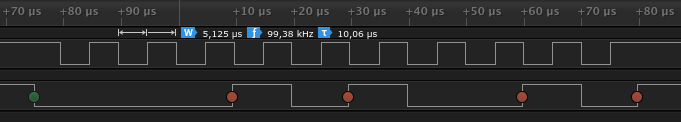
\includegraphics[width=0.8\linewidth]{3-edison_i2c6.png}
    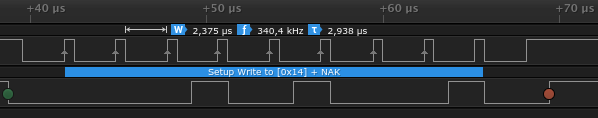
\includegraphics[width=0.8\linewidth]{3-edison_i2c1.png}
  \end{center}
  \caption{I2C port 6 exposed on custom expansion board not working.}
  \label{fig:endpoint_i2c16}
\end{figure}

After \ac{I2C} communication was working, additional wire for position sensing was connected to the pin 31. This pin is labeled as GPIO-44 on Intel Edison. To distribute \ac{I2C} addresses to the sensor node network first a general call is issued by addressing 0x00. To reset node addresses, 0x55 is sent. All of the listening nodes switch their address to a default value of 0x55 and set their position sensing pin output to low. After that, endpoint rises its position sensing pin to high and writes 0x11 into register 0xfa of address 0x55. Node which is directly connected to the endpoint will have its position sensing pin input set to high and will set its address to 0x11. To confirm that address was successfully set, endpoint reads from register 0xfa of address 0x11. If it receives 0x11 as an answer, address was successfully set and will pull the position sensing pin down. Then, it will write 0x01 to register 0xf0 of the node 0x11 which means that addressed node has to set its position sensing output pin high. After that endpoint does the same procedure for the next node increasing the number of the issued address. An edge condition is recognized by node not responding to read of its address. For example, if node 7 doesn't exist, reading from register 0xfa of address 0x17 won't return anything. Endpoint has a timeout and will detect that and set the position sensing output of the last addressed node back to low. The whole process can be seen in Figure \ref{fig:endpoint_sequence}.

\begin{figure}[h]
  \begin{center}
    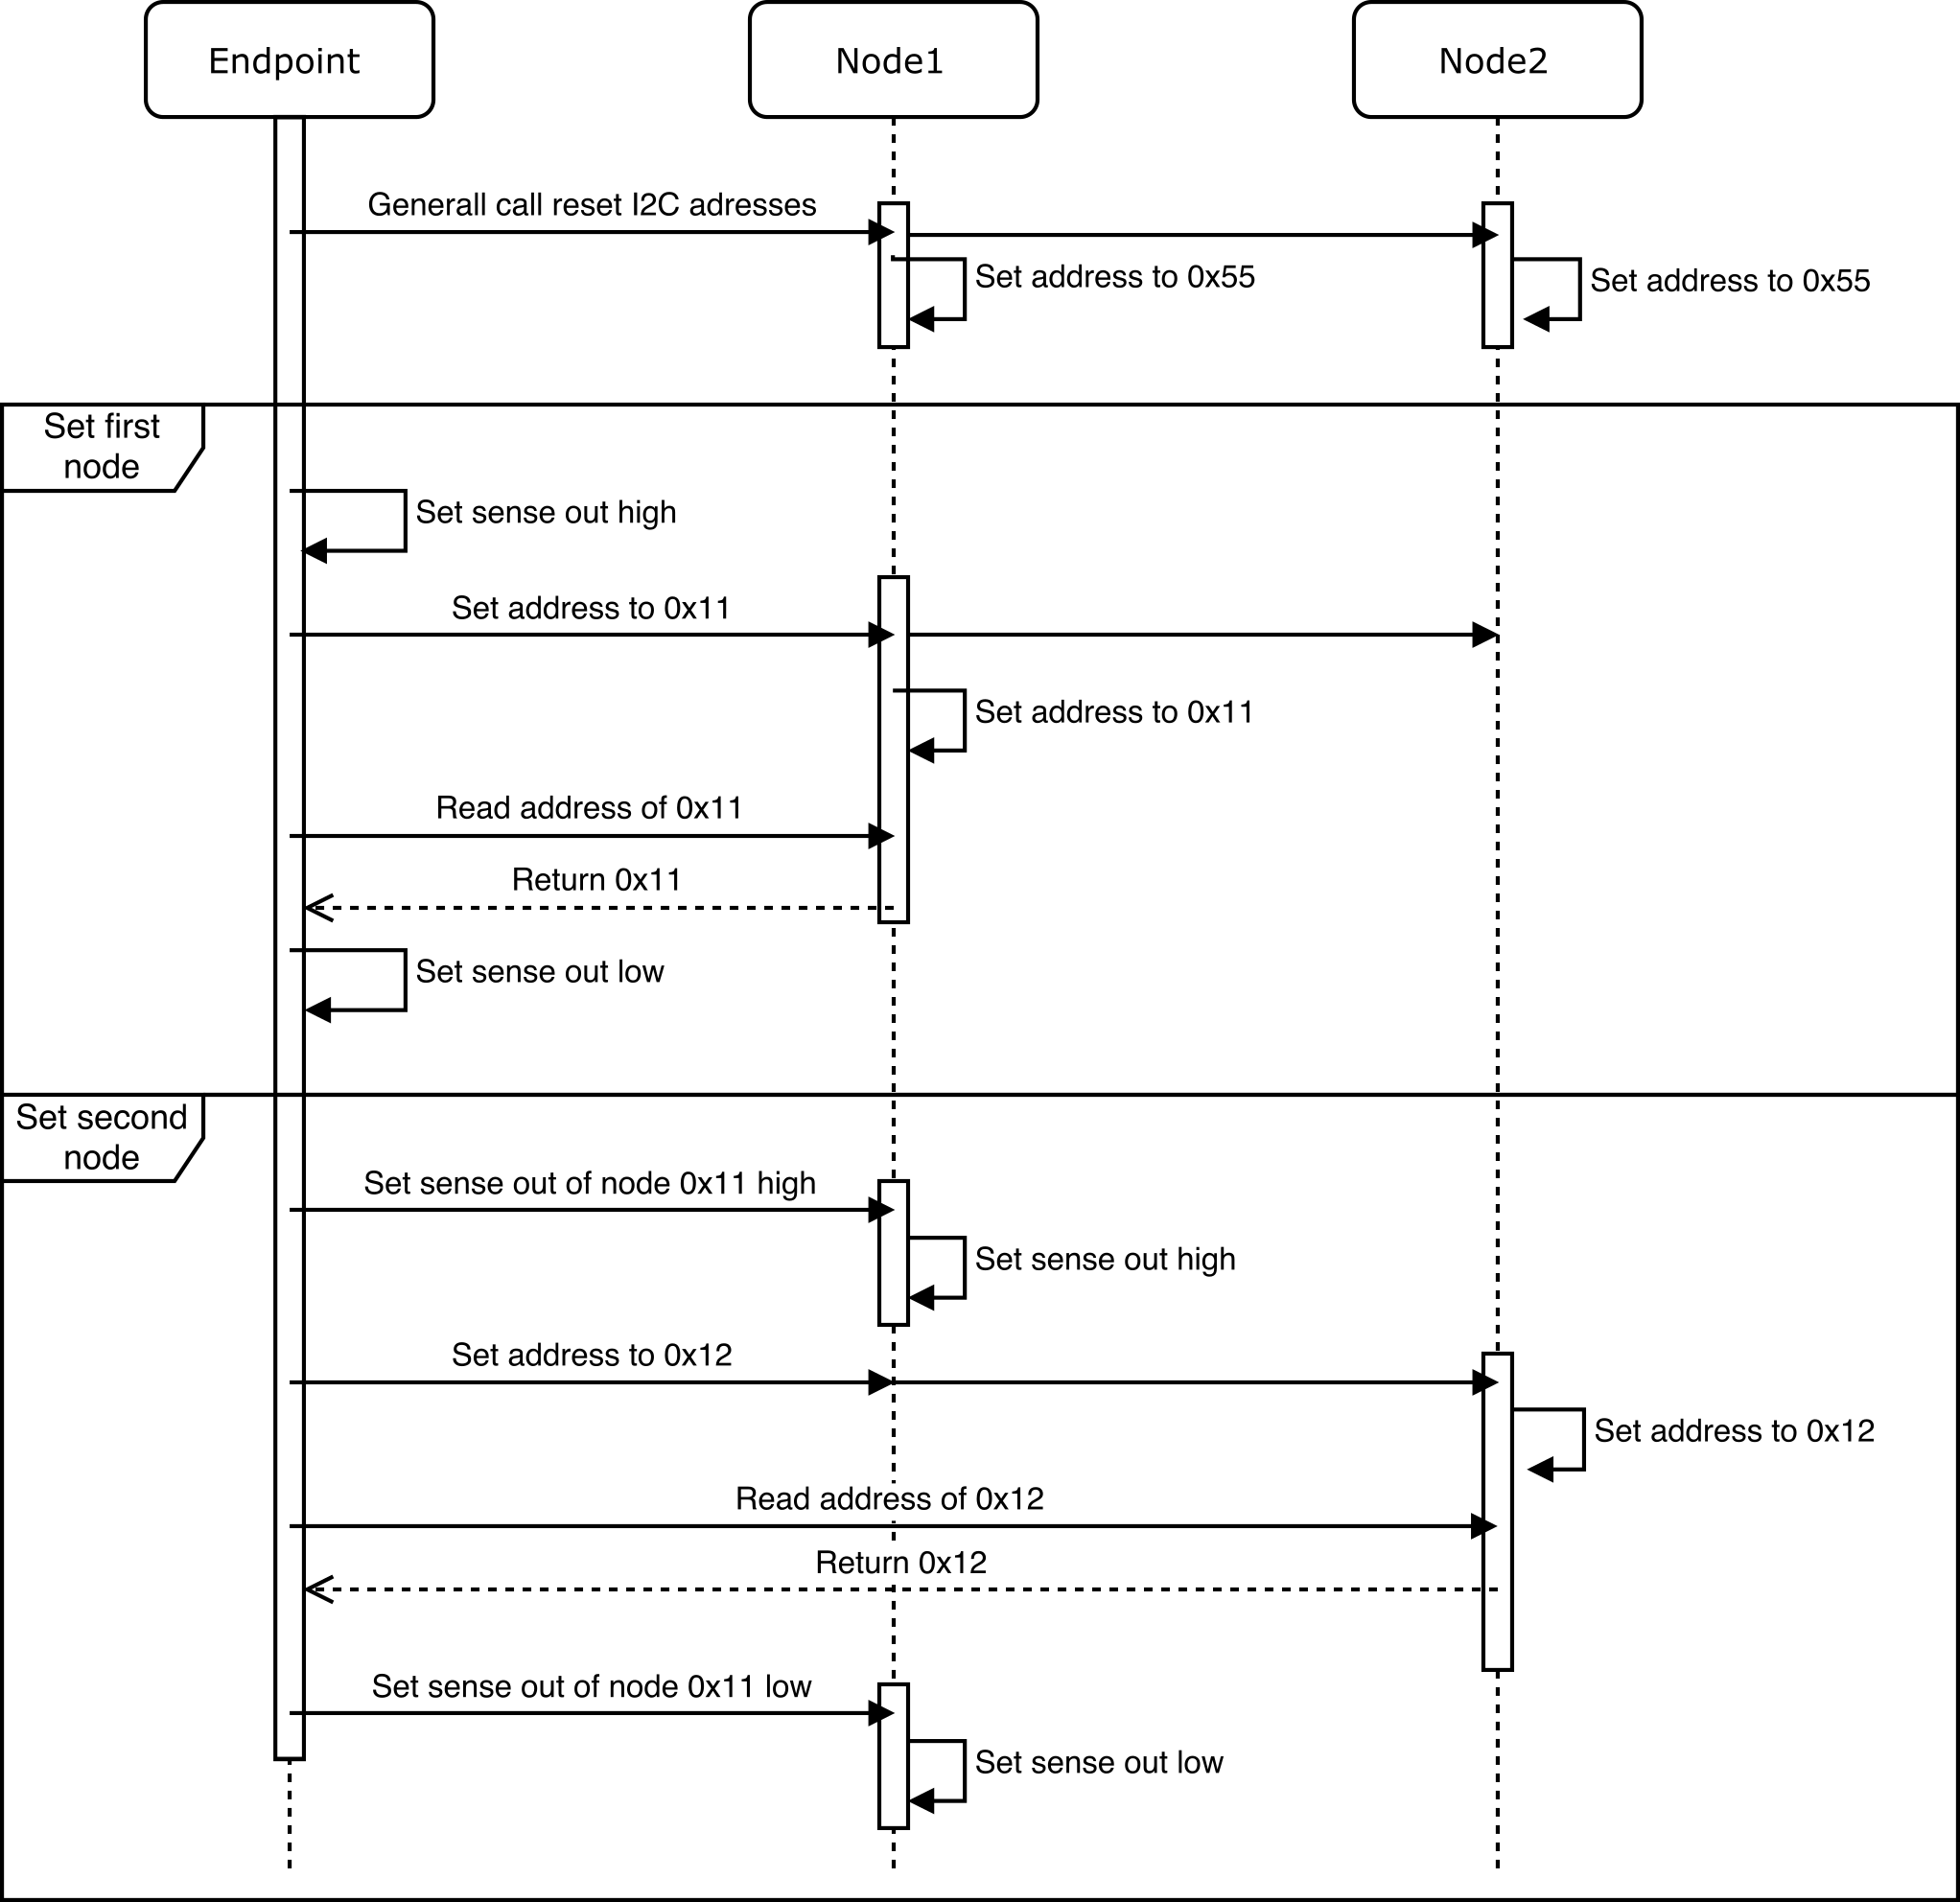
\includegraphics[width=\linewidth]{3-edison_sequence.png}
  \end{center}
  \caption{Sequence diagram showing process of address renewal for 2 nodes.}
  \label{fig:endpoint_sequence}
\end{figure}

\section{Data acquisition routine}
